\chapter{Using coordinates}
{ }\hfill\textbf{Level:} Newbie
\section{Presentation}
\noindent In this chapter, we're going to discover the primitive \texttt{setposition, setpos}. The drawing area has two axis that allows to determine each point using the cartesian coordinate system. The origin is the center of the drawing area. \\ \\ \\
\texttt{seposition list}\hspace {4cm } \textcolor{red}{ \texttt{setpos [100 -250]}}\\
 Moves the turtle to the co-ordinates specified by the two numbers in the list\\ \\
A little exemple:\\ 
\texttt{cs setpos [200 100] setpos [50 -150] setpos [-100 -150]}
\begin{center}
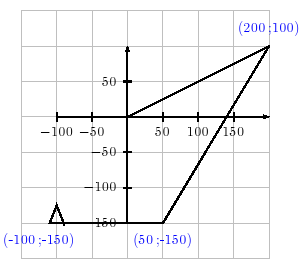
\includegraphics[scale=0.7]{pics/fpos-coord.png}
\end{center}
\vfill
\section{Exercice:}
\noindent
Try to draw this picture using only the following primitives: \texttt{setpos}, \texttt{cs}, \texttt{pu}, \texttt{pd}.\\
\begin{center}
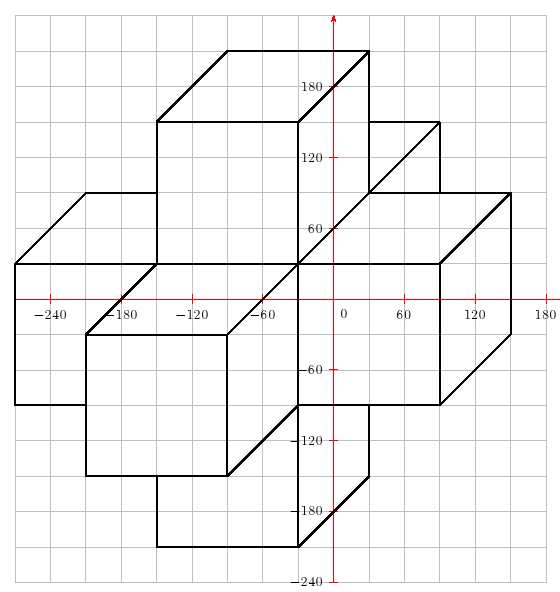
\includegraphics[scale=0.7]{pics/fpos-cube.png}
\end{center}